\section{Experiments and Results}
Description generall
limiations of work

\subsection{Extending the network}
The first round of experiments is dedicated to find out what 'conditions' the network seperates.
During an exploratory phase, some scenarios where the network indeed seperates were found.
Yet, they were sparse and could not be easily interpreted.
Therefore, in this step the knowledge gained from the initial experiments is put to use.
A systematic evaluation on the relationship between network size and splitting behaviour was conducted.

To enable comparisson between networks of different sizes, the network extension technique described in REF was used.
First, an extensive experiment with a network architecture of 4-8-8-2 was conducted.
To expand the range of the results, two additional experiments were executed, which were slightly smaller to lower computational cost.
One experiment is done on a network with only one hidden layer, concretely with a shape 4-20-2, and the other experiment on a network with three hidden layers, a shape of 4-4-4-4-2.
All hyperparameters are shared amongst the three experiments.
The only difference is the pruning target, which is derived from the network architecture.

For all three experiments, the pruning rate was set to $0.32$.
The chosen value, while somewhat arbitrary, was selected by promising results on preliminary tests.
\textcite{DBLP:conf/iclr/FrankleC19} used a pruning rate of $0.2$ in the original experiments for the fully connected feed forward network trained on the MNIST dataset.
However with a larger pruning rate, a larger space of network sizes can be covered with the same number of iterations, which is why the larger pruning rate of $0.32$ was selected.

\begin{table}[]
    \centering
    \resizebox{\columnwidth}{!}{%
    \begin{tabular}{@{}ccccccc@{}}
    \toprule
    \textbf{} & \multicolumn{2}{c}{one hidden layer} & \multicolumn{2}{c}{two hidden layers} & \multicolumn{2}{c}{three hidden layers} \\ \midrule
    \multicolumn{1}{|c|}{extension-level} & \multicolumn{1}{c|}{hidden dim} & \multicolumn{1}{c|}{\#param} & \multicolumn{1}{c|}{hidden dim} & \multicolumn{1}{c|}{\#param} & \multicolumn{1}{c|}{hidden dim} & \multicolumn{1}{c|}{\#params} \\ \midrule
    \multicolumn{1}{|c|}{0 (base)} & 20 & \multicolumn{1}{c|}{120} & 8 & \multicolumn{1}{c|}{112} & 4 & \multicolumn{1}{c|}{56} \\ \midrule
    \multicolumn{1}{|c|}{1} & 29 & \multicolumn{1}{c|}{174} & 10 & \multicolumn{1}{c|}{160} & 5 & \multicolumn{1}{c|}{80} \\ \midrule
    \multicolumn{1}{|c|}{2} & 43 & \multicolumn{1}{c|}{258} & 13 & \multicolumn{1}{c|}{247} & 6 & \multicolumn{1}{c|}{108} \\ \midrule
    \multicolumn{1}{|c|}{3} & 64 & \multicolumn{1}{c|}{384} & 16 & \multicolumn{1}{c|}{352} & 8 & \multicolumn{1}{c|}{176} \\ \midrule
    \multicolumn{1}{|c|}{4} & 94 & \multicolumn{1}{c|}{564} & 20 & \multicolumn{1}{c|}{520} & 10 & \multicolumn{1}{c|}{260} \\ \midrule
    \multicolumn{1}{|c|}{5} & 138 & \multicolumn{1}{c|}{828} & 25 & \multicolumn{1}{c|}{775} & 12 & \multicolumn{1}{c|}{360} \\ \midrule
    \multicolumn{1}{|c|}{6} & 202 & \multicolumn{1}{c|}{1212} & 31 & \multicolumn{1}{c|}{1147} & 15 & \multicolumn{1}{c|}{540} \\ \midrule
    \multicolumn{1}{|c|}{7} & 297 & \multicolumn{1}{c|}{1782} & 38 & \multicolumn{1}{c|}{1672} & 19 & \multicolumn{1}{c|}{836} \\ \midrule
    \multicolumn{1}{|c|}{8} & 437 & \multicolumn{1}{c|}{2622} & 47 & \multicolumn{1}{c|}{2491} & 23 & \multicolumn{1}{c|}{1196} \\ \midrule
    \multicolumn{1}{|c|}{9} & 643 & \multicolumn{1}{c|}{3858} & 57 & \multicolumn{1}{c|}{3591} & 29 & \multicolumn{1}{c|}{1856} \\ \midrule
    \multicolumn{1}{|c|}{10} & 946 & \multicolumn{1}{c|}{5676} & 70 & \multicolumn{1}{c|}{5320} & 35 & \multicolumn{1}{c|}{2660} \\ \midrule
    \multicolumn{1}{|c|}{11} & 1391 & \multicolumn{1}{c|}{8346} & 85 & \multicolumn{1}{c|}{7735} & 43 & \multicolumn{1}{c|}{3956} \\ \midrule
    \multicolumn{1}{|c|}{12} & 2046 & \multicolumn{1}{c|}{12276} & 104 & \multicolumn{1}{c|}{11440} & 52 & \multicolumn{1}{c|}{5720} \\ \midrule
    \multicolumn{1}{|c|}{13} & 3009 & \multicolumn{1}{c|}{18054} & 127 & \multicolumn{1}{c|}{16891} & 63 & \multicolumn{1}{c|}{8316} \\ \midrule
    \multicolumn{1}{|c|}{14} & 4425 & \multicolumn{1}{c|}{26550} & 154 & \multicolumn{1}{c|}{24640} & 77 & \multicolumn{1}{c|}{12320} \\ \midrule
    \multicolumn{1}{|c|}{15} &  & \multicolumn{1}{c|}{} & 188 & \multicolumn{1}{c|}{36472} & 94 & \multicolumn{1}{c|}{18236} \\ \midrule
    \multicolumn{1}{|c|}{16} &  & \multicolumn{1}{c|}{} & 229 & \multicolumn{1}{c|}{53815} & 114 & \multicolumn{1}{c|}{26676} \\ \midrule
    \multicolumn{1}{|c|}{17} &  & \multicolumn{1}{c|}{} & 278 & \multicolumn{1}{c|}{78952} &  & \multicolumn{1}{c|}{} \\ \midrule
    \multicolumn{1}{|c|}{18} &  & \multicolumn{1}{c|}{} & 337 & \multicolumn{1}{c|}{115591} &  & \multicolumn{1}{c|}{} \\ \midrule
    \multicolumn{1}{|c|}{19} &  & \multicolumn{1}{c|}{} & 410 & \multicolumn{1}{c|}{170560} &  & \multicolumn{1}{c|}{} \\ \midrule
    \multicolumn{1}{|c|}{20} &  & \multicolumn{1}{c|}{} & 498 & \multicolumn{1}{c|}{250992} &  & \multicolumn{1}{c|}{} \\ \midrule
    \multicolumn{1}{|c|}{21} &  & \multicolumn{1}{c|}{} & 604 & \multicolumn{1}{c|}{368440} &  & \multicolumn{1}{c|}{} \\ \midrule
    \multicolumn{1}{|c|}{22} &  & \multicolumn{1}{c|}{} & 733 & \multicolumn{1}{c|}{541687} &  & \multicolumn{1}{c|}{} \\ \midrule
    \multicolumn{1}{|c|}{23} &  & \multicolumn{1}{c|}{} & 890 & \multicolumn{1}{c|}{797440} &  & \multicolumn{1}{c|}{} \\ \midrule
    \multicolumn{1}{|c|}{24} &  & \multicolumn{1}{c|}{} & 1080 & \multicolumn{1}{c|}{1172880} &  & \multicolumn{1}{c|}{} \\ \midrule
    \multicolumn{1}{|c|}{25} &  & \multicolumn{1}{c|}{} & 1310 & \multicolumn{1}{c|}{1723960} &  & \multicolumn{1}{c|}{} \\ \bottomrule
    \end{tabular}%
    }
    \caption{In this table, the parameter trajectories and the corresponding hidden dimension of the network are displayed for each extension level. Parameter trajectory is in each respective 'param' column and the number of hidden neurons per hidden layer in the column 'hidden dim'. At the extension level zero, the base model values are displayed.}
    \label{tab:trajectory}
\end{table}

\subsubsection{Two hidden layers}
The first experiment was an extensive exploration of different model sizes by extending the network.
The base network, which is the network that is used as a base for extending, has the shape 4-8-8-2.
This architecture has 112 weights, which is also used as the pruning target.
The network architecture indicated by the number of neurons per hidden layer and the respective number of weights are displayed in \ref{tab:trajectory}.
The network is extended up to 25 times.
At the extension level 25, the network has a shape of 4-1310-1310-2, with 1.723.960 weights.
The number of extension levels corresponds to the number of pruning levels the network goes through.

Over all pruning levels, the network might seperate into two network or lose one of the inputs or outputs, which is called 'degrading'.
For the experiments described here, the run is stopped as soon as the network degrades to avoid unnecessary computational effort.
After each pruning level, the network is evaluated to check if it seperated or degraded.
When looking at this over the the course of all pruning levels, there are four different scenario for a network:
\begin{enumerate}
    \item seperated (and not degraded)\\
    The network seperates at some pruning level. 
    It does not degrade at any later level. 
    \item separated and later degraded \\
    The network splits at some point and has all input and output nodes.
    At a later level, the network degrades (it loses at least one input or output).
    \item degraded (and not seperate before) \\
    The network degrades before it can seperate.
    \item interconnected - not seperated and not degraged \\
    The network does neither seperate, nor degrade. 
    The result is a single network that contains all input and output nodes of all tasks.
\end{enumerate}
\begin{figure}[ht]
    \centering
    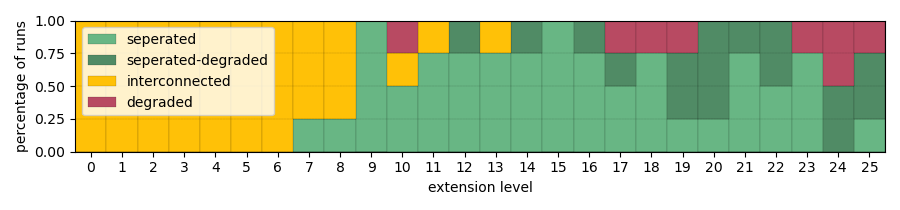
\includegraphics[width=1.0\linewidth]{2-layer-histogram-split-behaviour.png}
    \caption{Proportional Stacked Area Chart}
    \label{fig:2laxer-histogram}
\end{figure}

At each extension level, the runs are repeated with four different seeds for the network initialization.
The results are displayed in figure \ref{fig:2laxer-histogram}.
The figure is a proportional stacked area chart.
Each scenario described above is encoded with a color.
On the x-axis, the extension levels are shown.
On the y-axis, the percentage of networks in each category can be view.
A clear pattern in the data is, that the network seperates for the first time with at least 7 pruning levels.
The number of weights at that level is 1672, which is $~15$-times the amount of weights compared to the base model. 
Starting at extension level 9, which represents an increase of $~32$-times, the majority of the netowrks seperate.
Up until the 6-th extension level, no network seperates or degrades. 
However if the network would be pruned further, at some point every network would degrade.
Therefore it is also reasonable to assume that some of the networks that are still interconnected after all pruning iterations would seperate well, if they were pruned to less weights.

Another interesting observation is that only after extension level 10, the networks begin to degrade.
What follows from the data is, the more extension levels, the more likely it is that a network degrades, either before or after it seperated.

One possible explanation for this is that at each pruning level, a certain number of 'inactive weights' are produced.
As noted in \autocite{HanEtAl15, AllAlivePruning}, this is a known phenomenon.
However, since no regularisation is used in these experiments, the inactive weights do not decrease in magnitude.
Rather, they are frozen with they last value.
If more inactive parameters are created each pruning level than pruned, the percentage of inactive weights in the network grows over the iterations.
Therefore, the more pruning levels the network experienced, the less of its available, unpruned parameters are active.
This effectively makes the network smaller, which in turn makes it more likely to seperate or degrade.

\begin{figure}[ht]
    \centering
    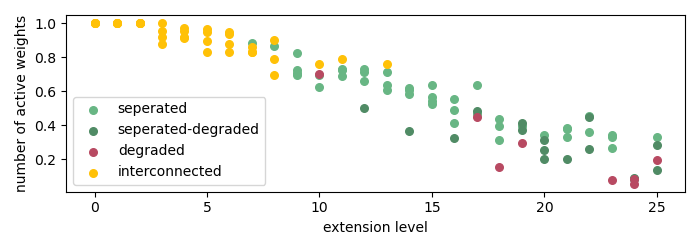
\includegraphics[width=1.0\linewidth]{2-layer-compund-damage.png}
    \caption{
        The figure depicts the number of active weights after the last pruning iteration of extended networks.
        On the x-axis, the extension level is displayed.
        On the y-axis, the number of active weights at that level.
        A clear pattern emerges, showing a correlation between number of pruning iterations and the number of active weights in the final network.
    }
    \label{fig:collateral_damage}
\end{figure}

This effect is visible in \ref{fig:collateral_damage}.
The colors are encoded in the same way as in \ref{fig:2laxer-histogram}.
Each dot is a single run. 
The x axis represents the extension level.
On the y-axis the number of active weights after the last pruning level is display.
Important to note is that since when a network degrades (red), the run is immediately stopped.
Therefore in this graph, the degraded networks might have larger numbers of active weights, compared to other networks that were pruned for the total amount of levels.
However even with this caveat, a clear trend is visible.
The more pruning levels the network experiences, the smaller the percentage of the networks weights that is active.
For some networks that were extended 20 or more levels, the final percentage of active weights in the network is only around $20$ percent, which translates to only $~22$ active weights.

Techniques like L1-Regularisation used in \autocite{HanEtAl15} or All alive Pruning \autocite{AllAlivePruning} could counteract this effect of compounding inactive parameters.
However, this is a topic for future research and not addressed in this thesis. 

\subsubsection{What makes the networks seperate?}
The question arises for what the main driver for splitting in this case is.

The model size or the number of pruning iterations.

To get a first impression and intuition about this question, a tangential experiment was launched with a grid of parameters.




\subsection{Extending the network}

The question arises for what the main driver for splitting in this case is.
The model size or the number of pruning iterations.
To get a first impression and intuition about this question, a tangential experiment was launched with a grid of parameters.
Four different network sizes and six different values for the number of pruning iterations are used, and each experiment is repeated four times with different seeds.
The network sizes $h \in \{31, 38, 48, 57\}$, where $h$ is the number of hidden neurons in the network with shape (4, h, h, 2).
The different number of pruning levels are $l = [1, 2, 3, 4, 5, 6, 7, 8, 9, 10]$.
This parameter range is similar to where the network first splits in the previous experiment.
For each network it is tracked if it splits.
\begin{figure}[ht]
    \centering
    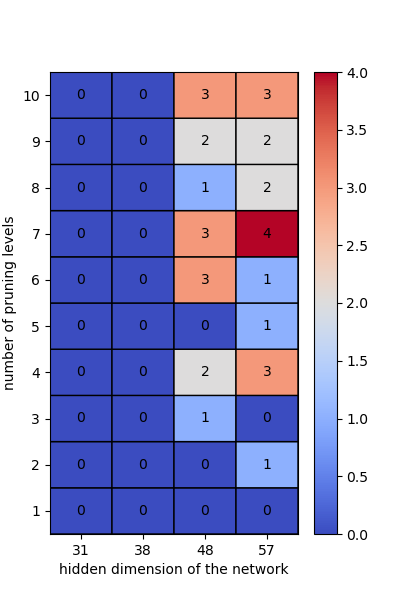
\includegraphics[width=1.0\linewidth]{grid.png}
    \caption{ef}
    \label{fig:grid}
\end{figure}

In figure \ref{fig:grid} the results are depicted as a heatmap. 
One can clearly see that in the case of the smaller network, increasing the number of pruning iterations from 6 in the case of the network with $h=31$ to 10 did not result in a split.
For completeness, also pruning levels between 1 and 5 did not lead the the network splitting.
For the network with $h=38$ also no splitting occurred over the whole range of pruning levels.
Starting at $h=48$, the network splits quite reliably.
Even with only $3$ pruning levels, one of the four networks split.

As for the network with $h=57$ a similar scenario plays out
The network splits for all tested number of pruning levels except for one-shot pruning, meaning only one pruning level.
The results suggest that the size of the network is a more important factor than the number of pruning levels, regarding network splitting.
Though, the results also show that the networks tend to split more often, when there are more pruning levels.

\begin{figure}[ht]
    \centering
    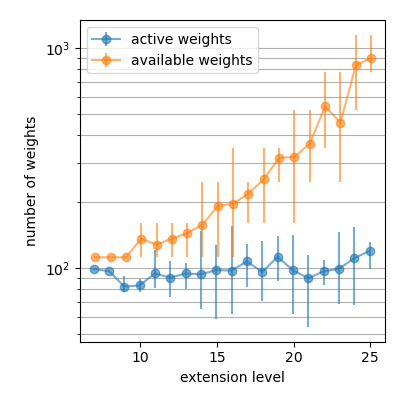
\includegraphics[width=.5\linewidth]{2-layer-active-available-at-split-log.png}
    \caption{
        The figure depicts the number of available weights / prunable weights (orange) and the number of active weights (blue) at the iteration when the networks first split.
        Each dot represents an average over four runs with different seeds.
        The error bars indicate the maximum and minimum value of the different runs.
        While the number of available weights at the split iteration increases, the number of active weights stays fairly constant.
        Logarithmic.
    }
    \label{fig:active-split}
\end{figure}

When the network size and the number of pruning levels is increased, the networks tend to split in earlier pruning levels.
This is indicated by the number of prunable weights the network has by the time it splits.
This is depicted in figure \ref{fig:active-split} by the organge line. 
Each point represents an average over four runs with different seeds for the model initialization. 

The networks tend to split earlier when they are larger.
Further, the number of active weights at the iteration slightly decreases as the networks get larger.

In these experiments, the networks tend to split in a narrow range of active weights in the network.
The largest number of active weights is 119 and the lowest is 82 at the iteration where the network splits.

To set this observation into more context, the same experiment was conducted for 2 additional architectures.
Once for a network with a single hidden layer, and once for a network with 3 hidden layers.
The networks were also extended like in the previously described experiment.
Each architecture was tested with 5 different seeds.

\subsubsection{Three hidden layers}
For this experiment, the base network has the shape (4, 6, 6, 6, 2).
This architecture has 108 weights, similar to the 120 from the previous example.
The network is extended for 15 levels, resulting in the largest shape of (4, ).
The full trajectory of the parameters is visible in refTABLE.

\begin{figure}[ht]
    \centering
    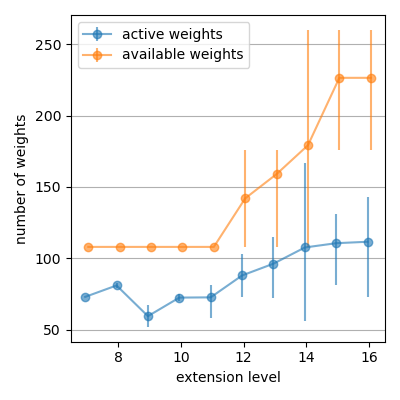
\includegraphics[width=.5\linewidth]{3-layer-active-available-at-split.png}
    \caption{
        The figure depicts the number of available weights / prunable weights (orange) and the number of active weights (blue) at the iteration when the networks first degrades.
        Each dot represents an average over five runs with different seeds.
        The error bars indicate the maximum and minimum value of the different runs.
        TODO: describe 
    }
    \label{fig:active-split-3layer}
\end{figure}

In figure \ref{fig:active-split-3layer} the results for the network with three hidden layers is displayed. 
The line represent the available weights and the active weights at the network after each pruning level.
Only the range of extension levels where the network seperated are displayed.
In this case, both metrics tend higher when increasing the model size.
Notably, the number of active weights is lower than in the case of the network with two hidden layers.
This might be the due to the slightly lower pruning target which is determined by the model architecture.


This indicates that the network splits 


\subsubsection{Performance of Lottery tickets}
are there differences in the performance of lottery tickets when they split?

compare 